\setcounter{secnumdepth}{3}
\setcounter{tocdepth}{3}
\chapter{Thiết kế và thực hiện phần cứng}
\section{Thiết kế hệ thống}
\subsection{Tổng quan kiến trúc hệ thống}
\begin{figure}[H]
    \centering
    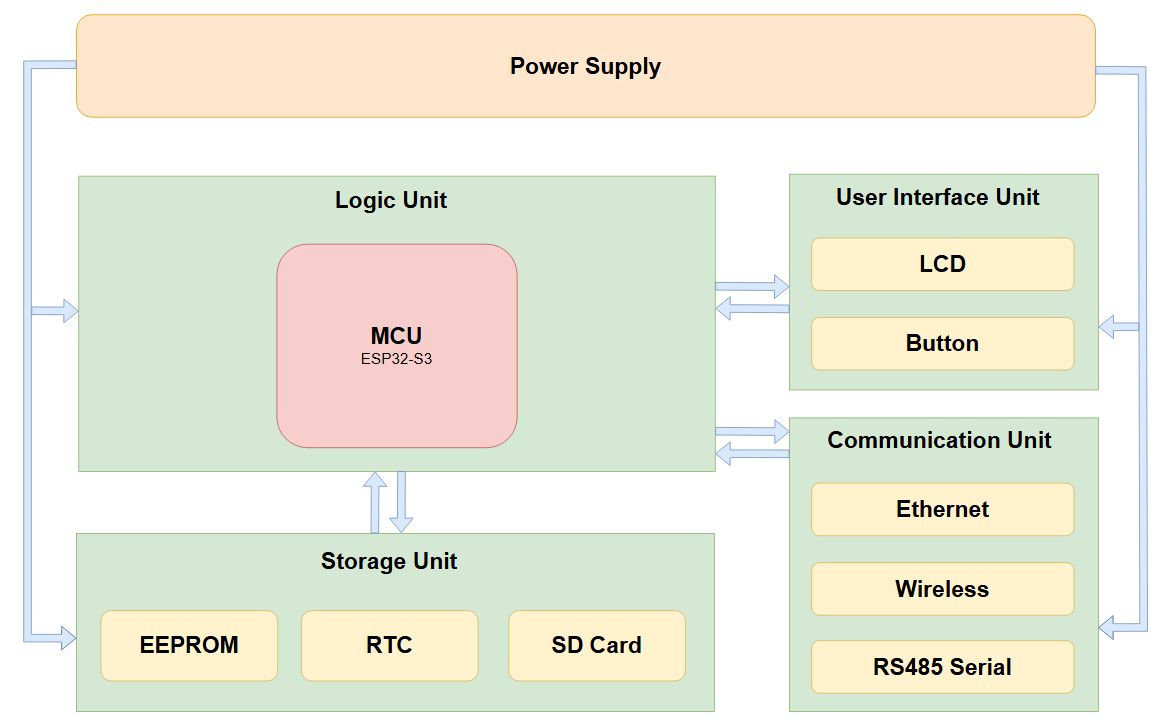
\includegraphics[width=0.9\textwidth]{image/so_do_khoi_tong_quat.png}
    \caption{Sơ đồ khối tổng quát thực hiện phần cứng}
    \label{fig:so_do_khoi_tong_quat}
\end{figure}
\textbf{Khối nguồn (Power Supply)}: có vai trò hạ áp từ nguồn một chiều DC 12-24V xuống mức 
5V và 3.3V để cung cấp điện cho các thành phần khác trong hệ thống, đảm bảo hoạt động
ổn định và an toàn. 

\textbf{Khối vi điều khiển xử lý trong tâm (Logic Unit)}: sử dụng ESP32-S3 được cung cấp khả năng tích hợp WiFi và BLE
Xử lý các tác vụ chính của hệ thống, đảm nhận các nhiệm vụ sau:
\begin{itemize}
    \item Giao tiếp với các thiết bị ngoại vi như LCD, module RS485, RTC và EEPROM thông qua các giao thức SPI, I2C và UART.
    \item Thu thập dữ liệu từ các thiết bị giám sát (Inverter, Meter, Weather Station) qua giao thức Modbus RTU qua RS485.
    \item Giao tiếp với web hiển thị dữ liệu thông qua giao thức MQTT.
\end{itemize}

\textbf{Khối lưu trữ (Storage Unit)}: tổ chức lưu trữ các dữ liệu như dữ liệu thu thập được, thông tin cấu hình 
wifi, cụ thể mỗi phần đảm nhận các nhiệm vụ sau:
\begin{itemize}
    \item Khối RTC (Real-Time Clock): sử dụng module DS3231 để cung cấp thời gian chính xác cho hệ thống, hỗ trợ việc đánh dấu 
thời gian cho dữ liệu thu thập và đồng bộ hóa với Server.
    \item Khối EEPROM: sử dụng module 24C256 để lưu trữ dữ liệu tạm thời khi mất kết nối mạng hoặc khi cần lưu trữ các thông 
số cấu hình của hệ thống như thông tin kết nối wifi,...
    \item Khối SD Card: được sử dụng để lưu trữ dữ liệu thu thập được từ các thiết bị kèm theo thời gian ghi nhận.
\end{itemize}

\textbf{Khối giao tiếp (Communication Unit)}: bao gồm các giao thức truyền thông:
\begin{itemize}
    \item Giao tiếp Modbus RTU qua RS485: để thu thập dữ liệu từ các thiết bị giám sát năng lượng điện Power Meter. 
    Giao thức này được lựa chọn do tính ổn định và khả năng truyền dữ liệu ở khoảng cách xa trong môi trường công nghiệp.
    \item Giao tiếp BLE: Được sử dụng để nhận cấu hình từ App của người dùng gửi xuống.
    \item Giao tiếp MQTT: sử dụng kết nối wifi 2.4GHz hoặc thông qua cổng Ethernet để truyền dữ liệu định kỳ theo thời gian đến web hiển thị, giúp người 
    dùng có thể theo dõi tình trạng hệ thống một cách trực quan và kịp thời.
\end{itemize}

\textbf{Khối giao tiếp với người dùng (User Interface Unit)} bao gồm các thành phần:
\begin{itemize}
    \item LCD 16x04: hiển thị các thông số tổng quát về thiết bị.
    \item Nút nhấn và Encoder: để người dùng có thể tương tác, thay đổi thông số cấu hình cho thiết bị thông qua màn hình LCD
\end{itemize}

\subsection{Các khối chức năng chính của trong hệ thống}
\begin{figure}[H]
    \centering
    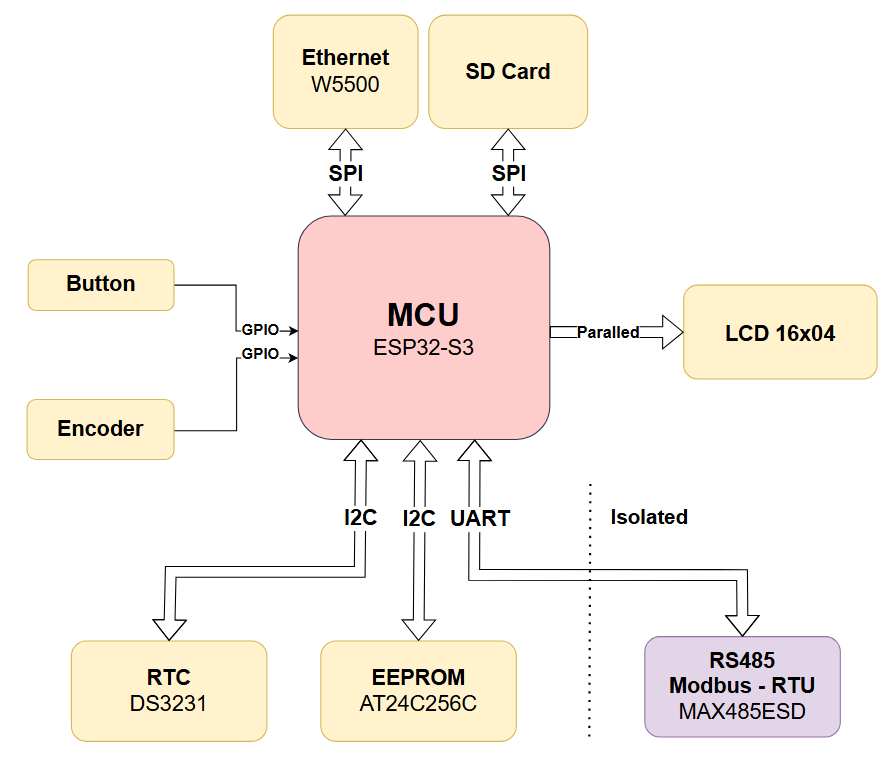
\includegraphics[width=0.9\textwidth]{image/so_do_luong_du_lieu.png}
    \caption{Sơ đồ khối tổng quát của phần cứng}
    \label{fig:so_do_luong_du_lieu}
\end{figure}
\begin{itemize}
    \item Dữ liệu từ các thiết bị giám sát (các Power Meter) được thu thập định kỳ thông qua giao thức Modbus RTU qua chuẩn vật lý RS485 và được xử lý bởi ESP32.
    \item Dữ liệu sau khi được xử lý sẽ được truyền về Server thông qua giao thức MQTT qua Ethernet hoặc Wi-Fi. Đồng thời, dữ liệu về tình trạng đường truyền
    cũng được truyền đến web hiển thị thông qua giao thức MQTT để người dùng có thể theo dõi tình trạng hệ thống một cách trực quan và kịp thời.
    \item Các thông số tổng như tổng công suất, tổng điện áp, tổng dòng điện,... sẽ được hiển thị trên LCD 16x04 để người dùng có thể theo dõi nhanh tình trạng hệ thống ngay tại chỗ.
    \item Người dùng có thể tương tác với hệ thống thông qua màn hình LCD hiển thị các thông số và các nút nhấn tùy chỉnh.
    \item Các thông số cấu hình như wifi sẽ được lưu trữ ở EEPROM, thiết bị sau khi khởi đông lại sẽ đọc các thông số cấu hình từ EEPROM để nạp lại cho hệ thống.
\end{itemize}


Cấu trúc Power Tree của hệ thống được thiết kế để đảm bảo nguồn điện được phân phối một cách hiệu quả và ổn định đến tất cả các thành phần, đồng thời cung cấp khả năng mở rộng trong tương lai nếu cần thiết.
\begin{figure}[H]
    \centering
    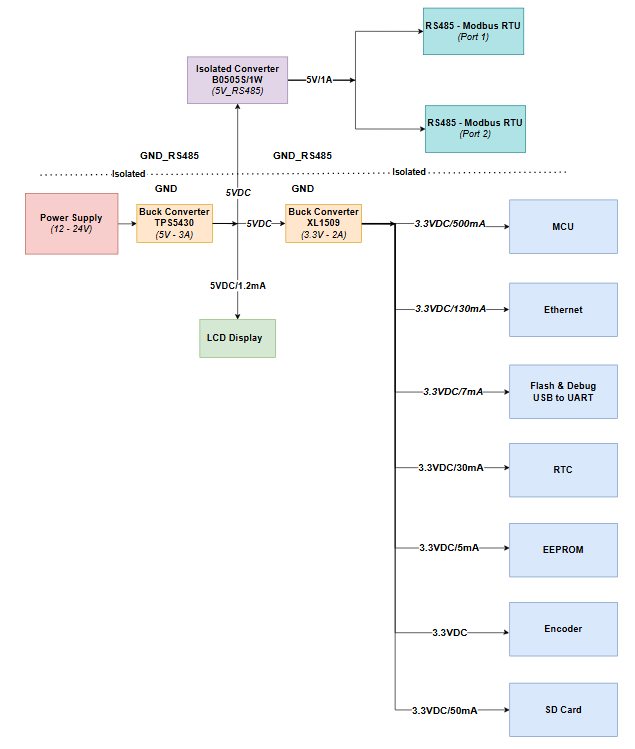
\includegraphics[width=1.05\textwidth]{image/power_tree.png}
    \caption{Sơ đồ khối phân bố nguồn trong hệ thống}
    \label{fig:power_tree}
\end{figure}
Nguồn DC 12-24V được đưa vào module hạ áp (buck converter) sử dụng IC TPS5430 
để tạo ra điện áp 5V. Từ nguồn 5V tiếp tục hạ áp xuống 3.3V thông qua IC XL1509
hoặc LDO để cấp cho các các khối khác và vi điều khiển, nguồn 3.3V được sử dụng chủ yếu 
trong hệ thống nên ta chọn IC XL1509 cho dòng ngõ ra ở khoảng rộng hơn (1-2A) thay vì sử dụng
LDO ngõ ra chỉ khoảng 1A.
\begin{itemize}
    \item \textbf{Nguồn 5V}: cấp cho LCD, khối cách ly RS485.
    \item \textbf{Nguồn 3.3V}: cấp cho vi điều khiển ESP32, module Ethernet, mạch debug cho ESP32,
module RTC, EEPROM và module SD Card.
\end{itemize}

\subsection{Chi tiết thiết kế phần cứng}
\subsubsection{Thiết kế khối vi điều khiển}
\begin{figure}[H]
    \centering
    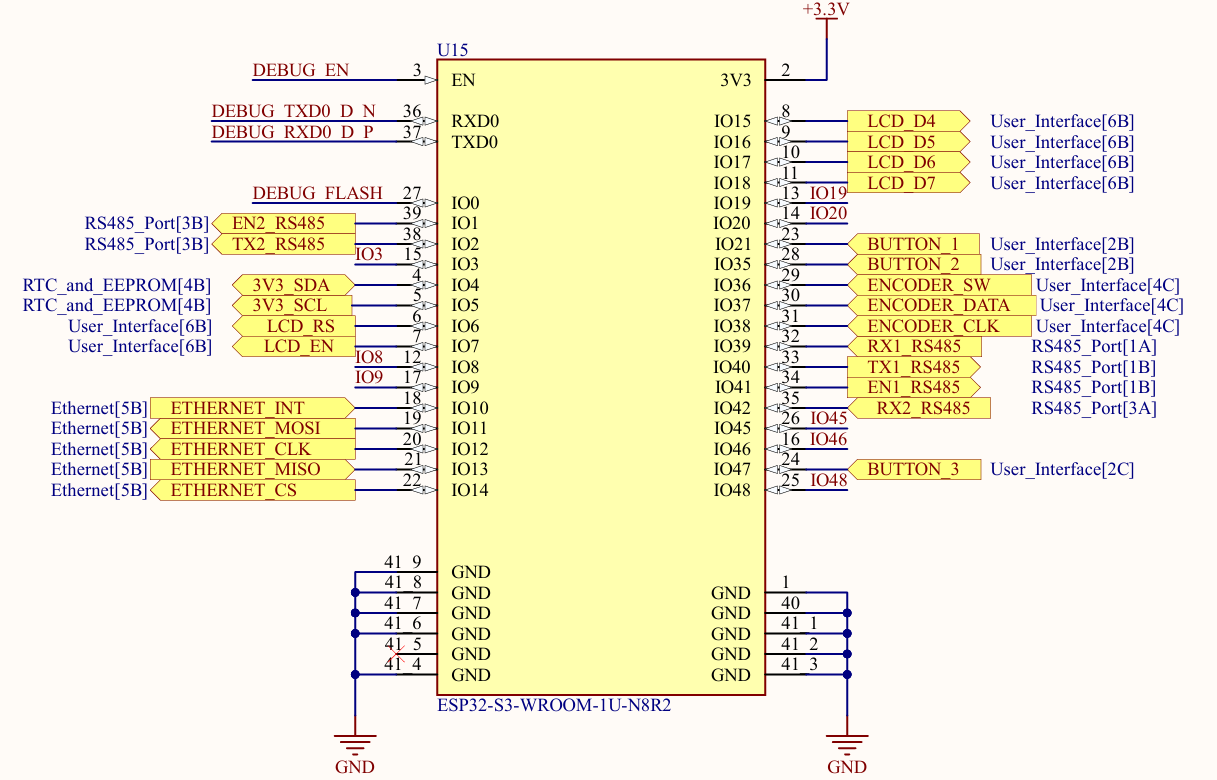
\includegraphics[width=1\textwidth]{image/mcu_esp32.png}
    \caption{khối vi điều khiển}
    \label{fig:mcu_esp32}
\end{figure}

Sử dụng ESP32-S3 N8R2 làm bộ xử lý trung tâm cho các tác vụ tại thiết bị thu thập dữ liệu, với dung lượng bố nhớ flash là 8MB và bộ nhớ RAM 2MB ngoại được tích hợp sẵn trong module, Vi điều khiển hỗ trợ các 
giao tiếp cơ bản như Wifi, Bluetooth/BLE giúp mở rộng khả năng giao tiếp trong quá trình phát triển thiết bị.
\begin{figure}[H]
    \centering
    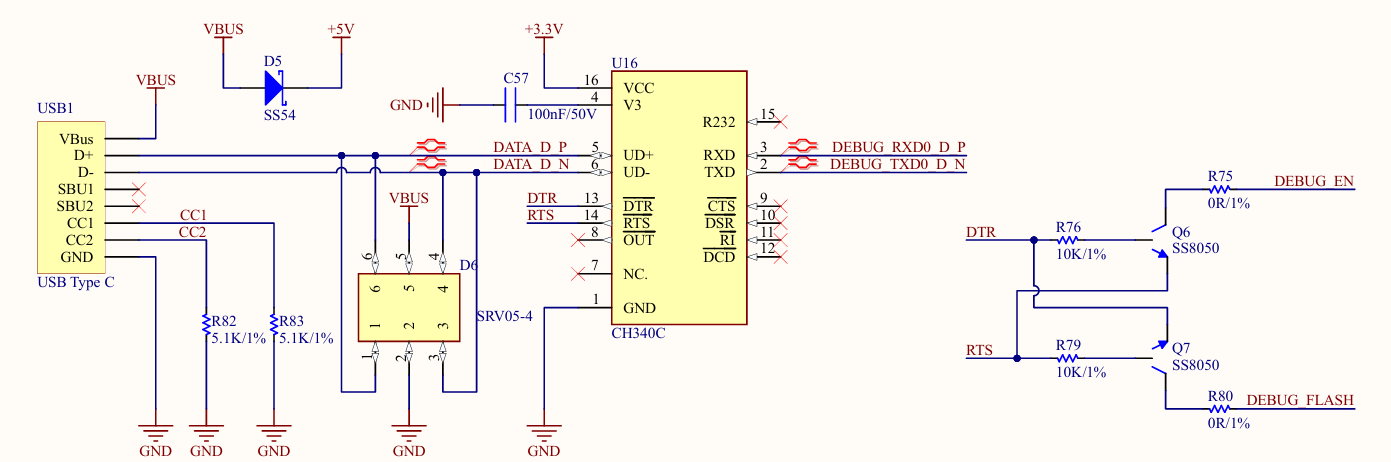
\includegraphics[width=1\textwidth]{image/debug_esp32.png}
    \caption{khối nạp code và Debug}
    \label{fig:mcu_esp32}
\end{figure}
Sử dụng IC CH340C làm IC debug chính cho thiết bị kết hợp với mạch nạp code tự động.

Cổng nạp sử dụng cổng type-C phổ biến và Diode giúp không cho điện áp cao từ board mạch truyền ngược lại vào máy tính.
\begin{figure}[H]
    \centering
    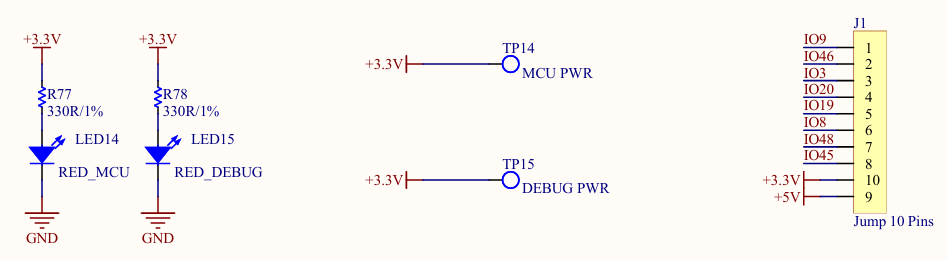
\includegraphics[width=0.95\textwidth]{image/led_esp32.png}
    \caption{khối kiểm tra nguồn cho vi điều khiển}
    \label{fig:mcu_esp32}
\end{figure}
Thiết kế hai đèn LED báo nguồn để người dùng có thể biết vi điều khiển đã có nguồn hay chưa.

Các chân chưa được sử dụng trong thiết kế mạch được đưa ra chân header giúp cho việc có thể phát triển trong tương lai.
\begin{figure}[H]
    \centering
    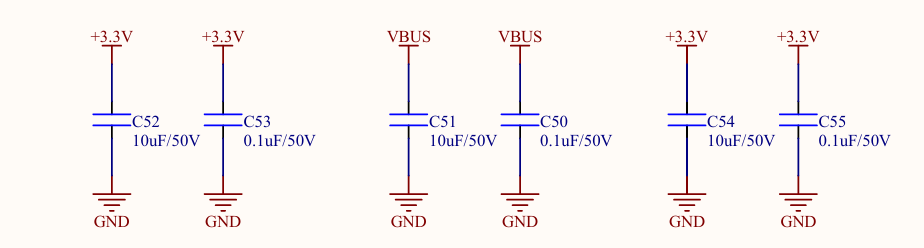
\includegraphics[width=0.95\textwidth]{image/esp_filter.png}
    \caption{khối lọc nguồn đầu vào cho vi điều khiển}
    \label{fig:esp_filter}
\end{figure}
Tích hợp thêm các tụ lọc nguồn đầu vào cho vi điều khiển, nhằm đảm bảo điện áp cấp vào cho vi điều khiển được ổn định quanh mức cho phép.

\subsubsection{Thiết kế khối nguồn}
\begin{figure}[H]
    \centering
    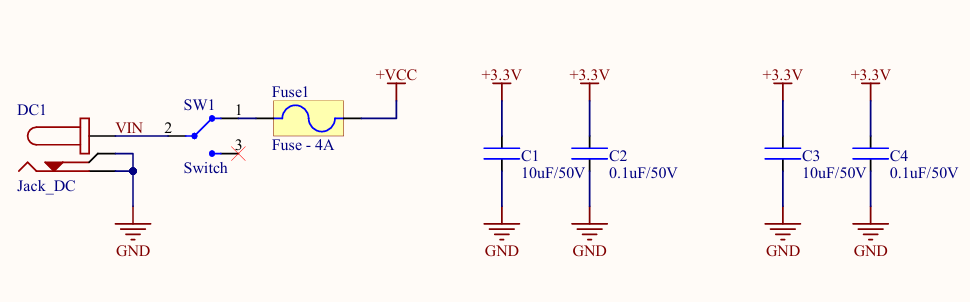
\includegraphics[width=0.95\textwidth]{image/dc_in.png}
    \caption{khối nguồn đầu vào}
    \label{fig:dc_in}
\end{figure}
Sử dụng Adapter 12VDC/3A để cấp nguồn cho thiết bị thông qua Jack DC, dải điện áp đầu vào mà thiết bị có thể hoạt động là 12-24VDC.

Mạch có tích hợp sử dụng cầu chì giúp bảo vệ mạch khi quá dòng và các tụ lọc nguồn đầu vào giúp ổn định điện áp cấp vào mạch. 
\begin{figure}[H]
    \centering
    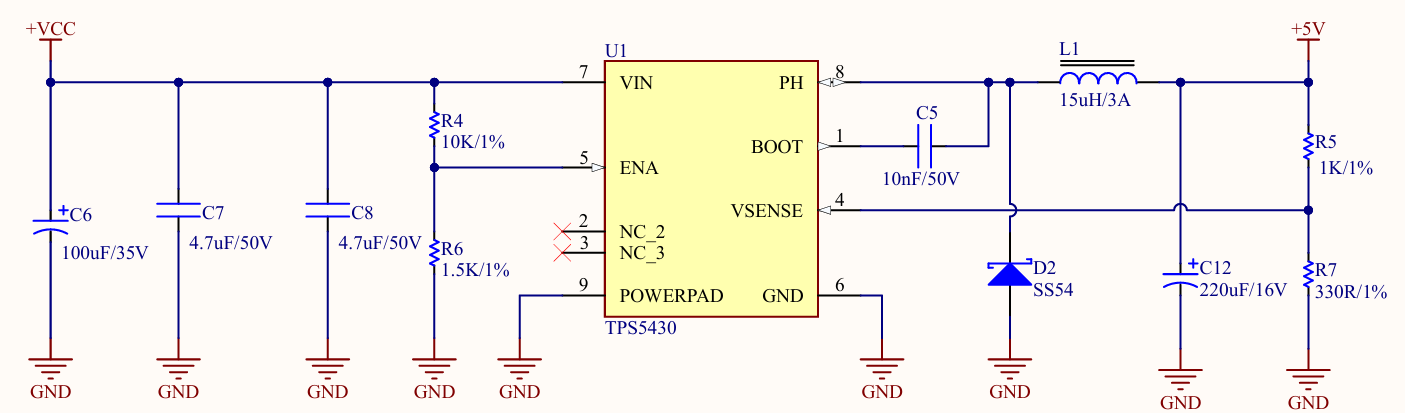
\includegraphics[width=0.95\textwidth]{image/buck_5v.png}
    \caption{Khối nguồn hạ áp 5V}
    \label{fig:buck_5v}
\end{figure}
Sử dụng IC TPS5430 để hạ áp xuống 5V/3A ổn định tại ngõ ra với các thông số linh kiện tham khảo theo datasheet của linh kiện.
\begin{figure}[H]
    \centering
    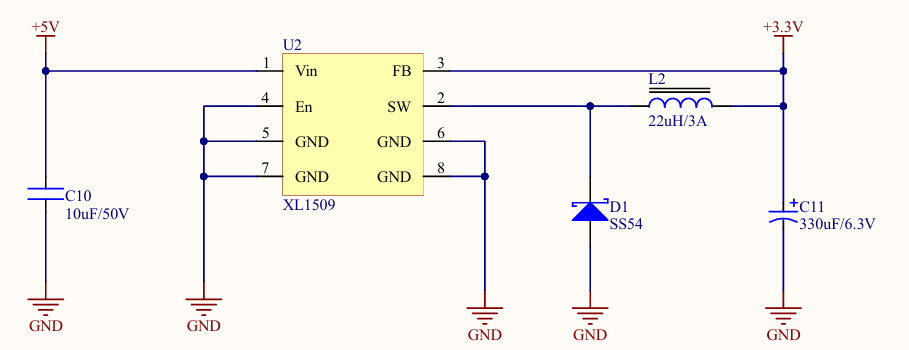
\includegraphics[width=0.95\textwidth]{image/buck_3v3.png}
    \caption{Khối nguồn hạ áp 3.3V}
    \label{fig:buck_3v3}
\end{figure}
Sử dụng IC XL1509 để hạ áp xuống 3.3V/2A với các thông số linh kiện tham khảo theo datasheet của linh kiện, đây là nơi cung cấp nguồn
chính cho các khối hoạt động trong mạch nên ta chọn IC cho dòng điện ngõ ra lớn hơn để có thể mở rộng sau này.
\begin{figure}[H]
    \centering
    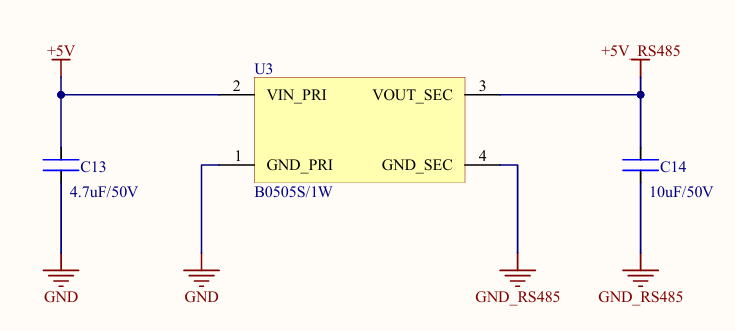
\includegraphics[width=0.95\textwidth]{image/isolated_5v.png}
    \caption{khối nguồn cách ly 5V}
    \label{fig:isolated_5v}
\end{figure}
Sử dụng trực tiếp nguồn 5V có trên mạch để thực hiện tạo ra nguồn cách ly cho khối giao tiếp RS485, mục đích của việc cách ly là giúp cho
các thành phần linh kiện trên mạch không bị tác động bởi các thiết bị bên ngoài kết nối với mạch thông qua khối RS485, tránh làm hỏng các
linh kiện có trên mạch khi có các gai điện áp cao đi thẳng vào mạch, các tụ lọc nguồn giúp ổn định điện áp đầu vào cho các thành phần chính
trong mạch hoạt động ổn định.
\begin{figure}[H]
    \centering
    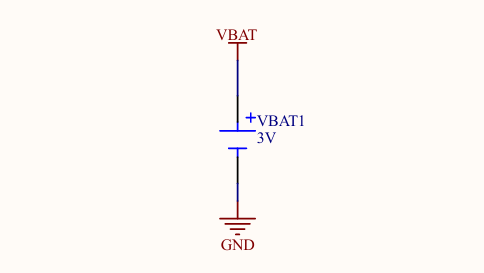
\includegraphics[width=0.5\textwidth]{image/pin_rtc.png}
    \caption{khối nguồn Pin rời cho mạch RTC}
    \label{fig:pin_rtc}
\end{figure}
Sử dụng nguồn từ pin CR2032 cung cấp cho khối RTC, khối RTC sẽ hoạt động với nguồn cấp từ mạch nếu có nguồn adapter cấp cho mạch, khi adapter 
không cấp nguồn cho mạch thì khối RTC sẽ vẫn hoạt động dựa trên pin CR2032 này nhằm đảm bảo khối RTC vẫn hoạt động bình thường, giúp cung cấp 
thời gian chính xác tới khi nguồn điện chính từ adapter được cấp lại.
\subsubsection{Thiết kế khối Ethernet}
\begin{figure}[H]
    \centering
    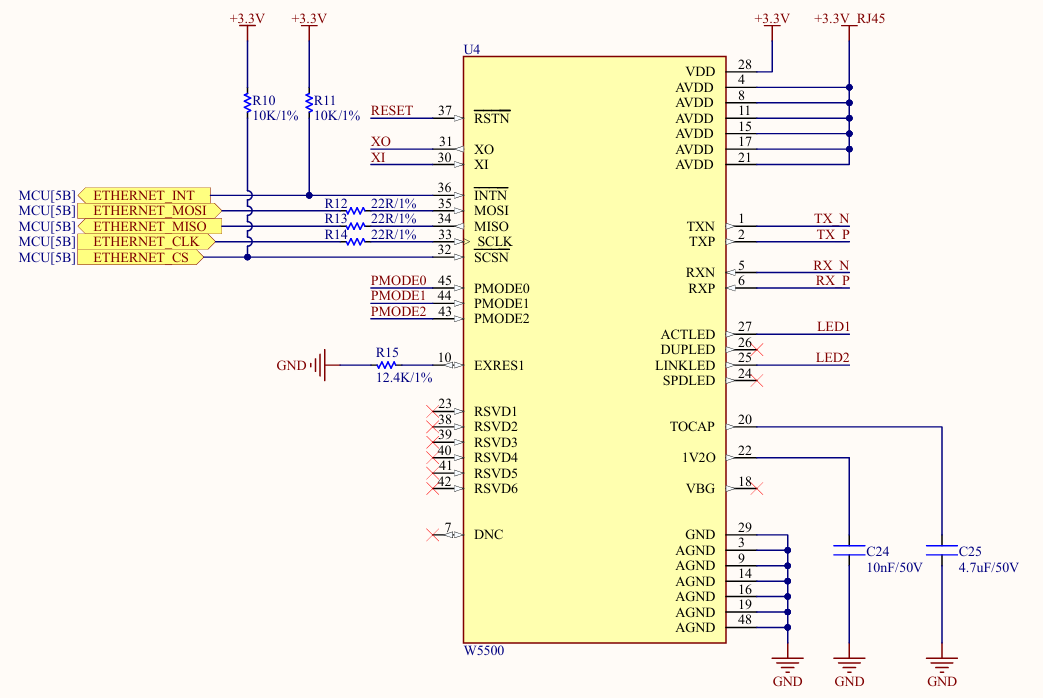
\includegraphics[width=1\textwidth]{image/w5500.png}
    \caption{khối vi điều khiển cho Ethernet}
    \label{fig:w5500}
\end{figure}
Sử dụng chip W5500 làm chip chính cho khối Ethernet, sử dụng W5500 ở chế độ Mac raw, tức là xử lý gói tin nhận/gửi ở layer 1 và layer 2.
\begin{figure}[H]
    \centering
    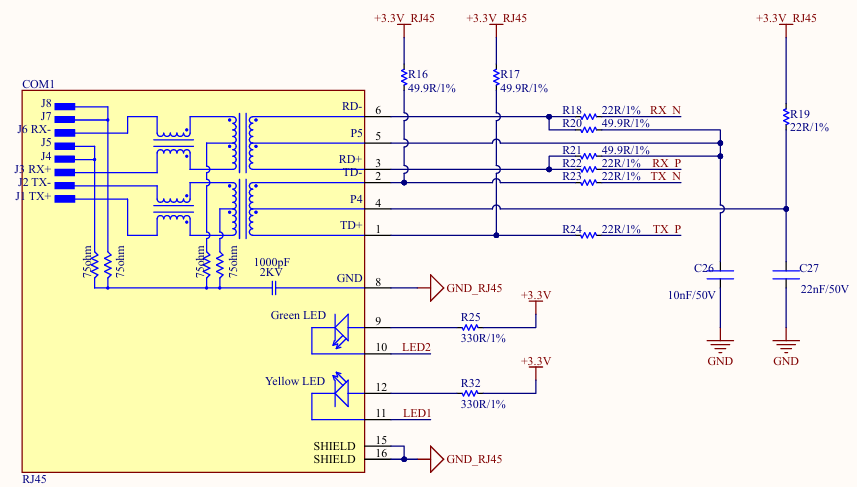
\includegraphics[width=1\textwidth]{image/rj45.png}
    \caption{khối cổng kết nối cho Ethernet}
    \label{fig:rj45}
\end{figure}
Cổng RJ45 được chọn để truyền/nhận gói tin cho giao tiếp Ethernet, sử dụng các điện trở kéo lên để giúp đường truyền tránh tình trạng floating,
các điện trở hạn dòng và 
\begin{figure}[H]
    \centering
    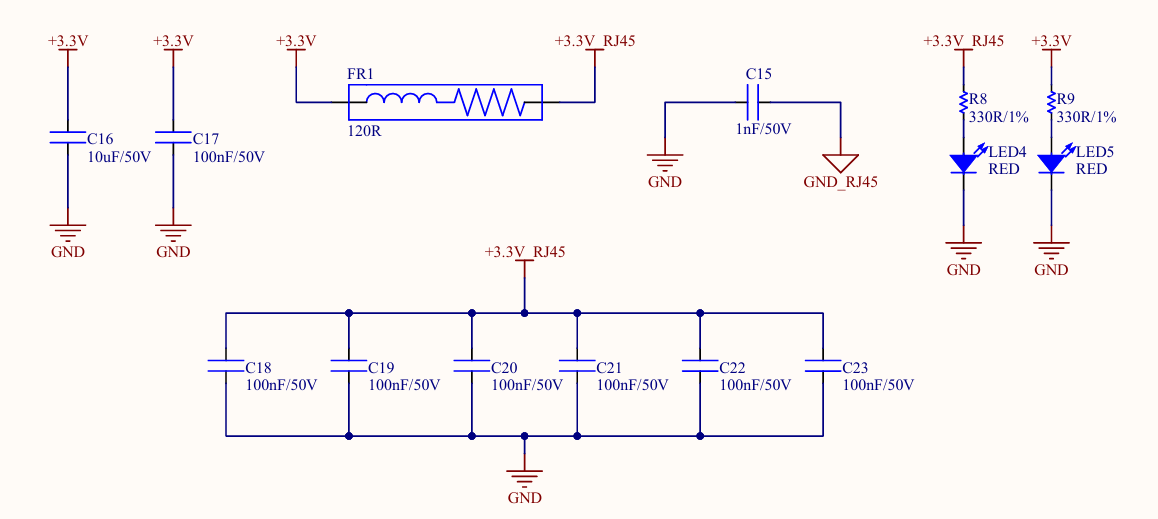
\includegraphics[width=0.7\textwidth]{image/filter_eth.png}
    \caption{khối lọc nguồn đầu vào cho Ethernet}
    \label{fig:filter_eth}
\end{figure}
\begin{figure}[H]
    \centering
    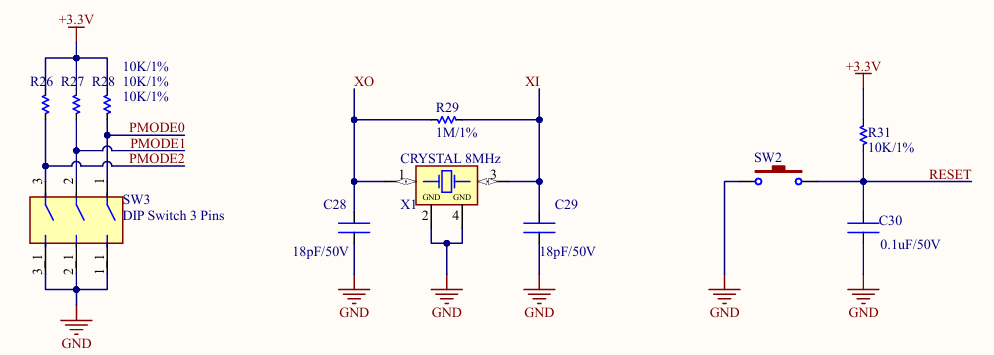
\includegraphics[width=0.7\textwidth]{image/eth_other.png}
    \caption{khối thạch anh và DIP Switch cho Ethernet}
    \label{fig:eth_other}
\end{figure}
Dip switch đóng vai trò trong việc chọn mode hoạt động cho chip Ethernet.
Thạch anh cung cấp xung clock 25MHz cho chip hoạt động.
Tích hợp nút reset khi chip bị treo hoặc có lỗi. 

\subsubsection{Thiết kế khối giao tiếp RS485}
\begin{figure}[H]
    \centering
    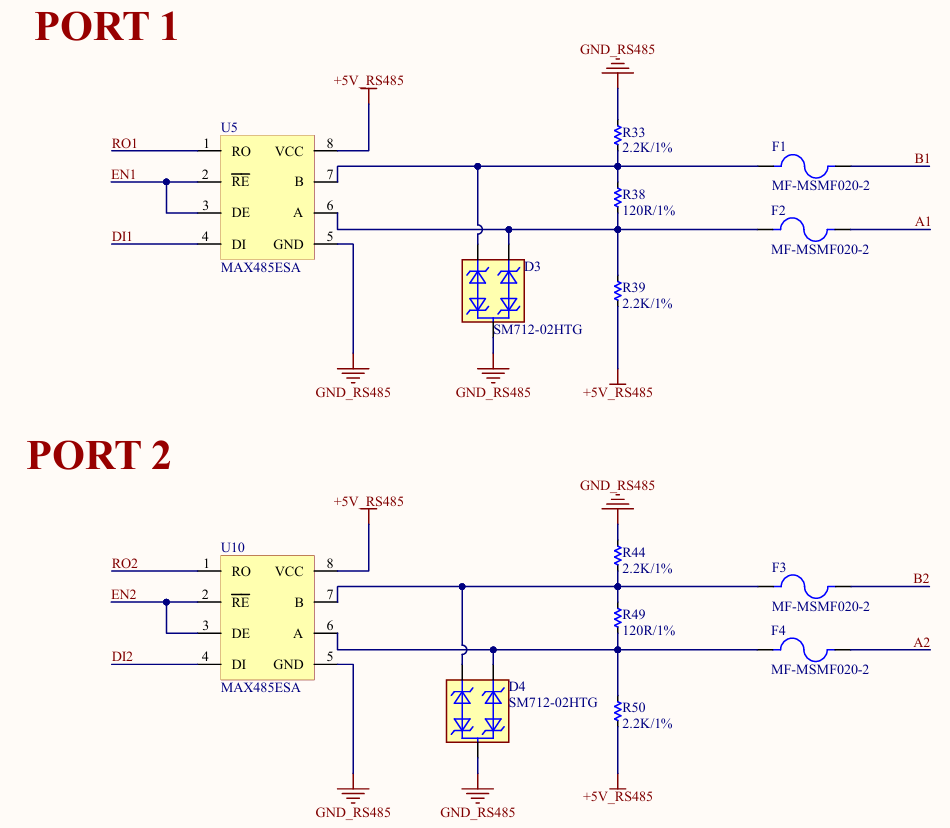
\includegraphics[width=0.9\textwidth]{image/rs485_max485.png}
    \caption{khối xử ly tín hiệu RS485}
    \label{fig:rs485_max485}
\end{figure}
IC MAX485 đóng vai tròng chính trong việc giao tiếp RS485 giữa vi điều khiển với các thiết bị modbus nói riêng và các thiết bị sử dụng chuẩn RS485.

Hai đường tín hiệu A và B có sử dụng điện trở kéo lên và kéo xuống giúp tránh tình trạng floating khi đường truyền rảnh.

Tích hợp hai cầu chì tự phục hồi với dòng điện định mức là 0.75A và TVS, giúp bảo vệ mạch bên trong trước các gai điện áp cao từ ngoài đưa vào mạch. 
\begin{figure}[H]
    \centering
    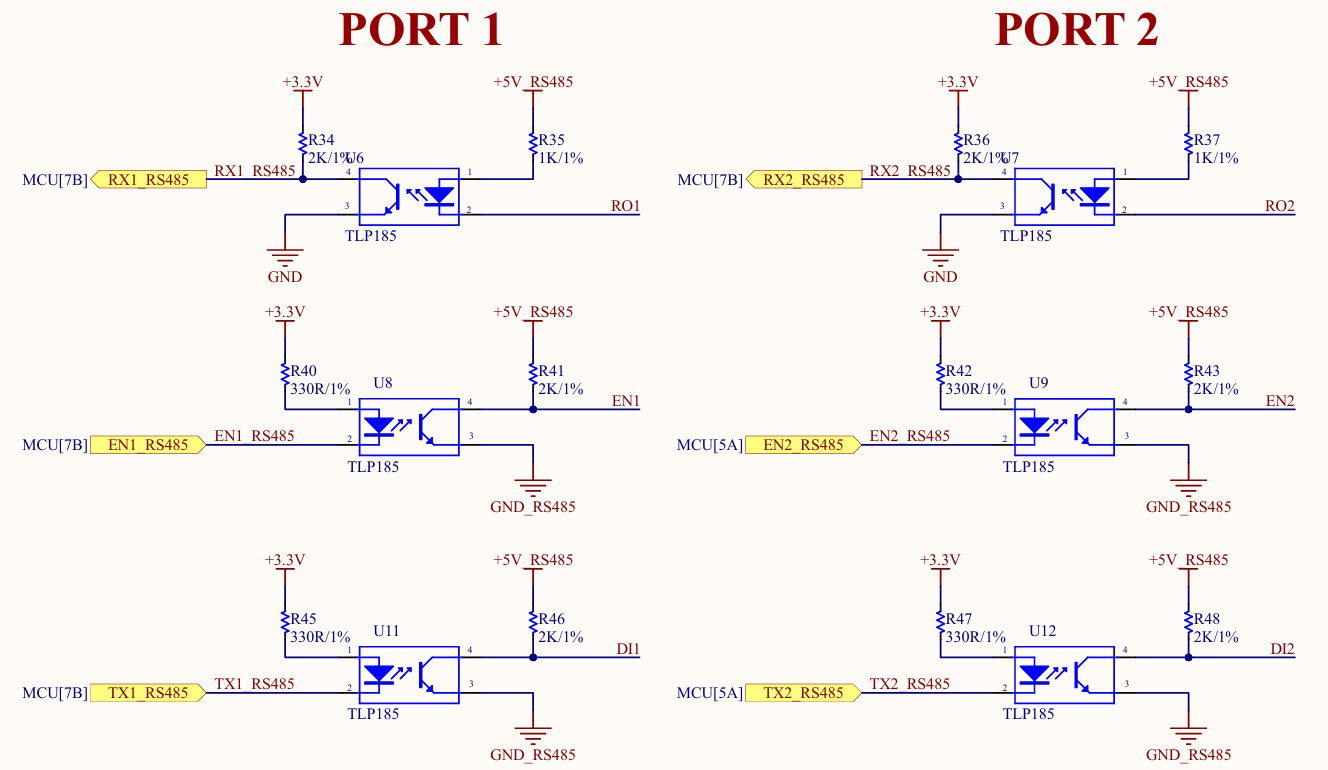
\includegraphics[width=0.9\textwidth]{image/rs485_opto.png}
    \caption{khối cách ly RS485}
    \label{fig:rs485_optp}
\end{figure}
Mạch sử dụng Opto quang giúp cách ly mạch chính với khối giao tiếp RS485, sử dụng các điện trở kéo lên giúp tránh tình trạng floating.
\begin{figure}[H]
    \centering
    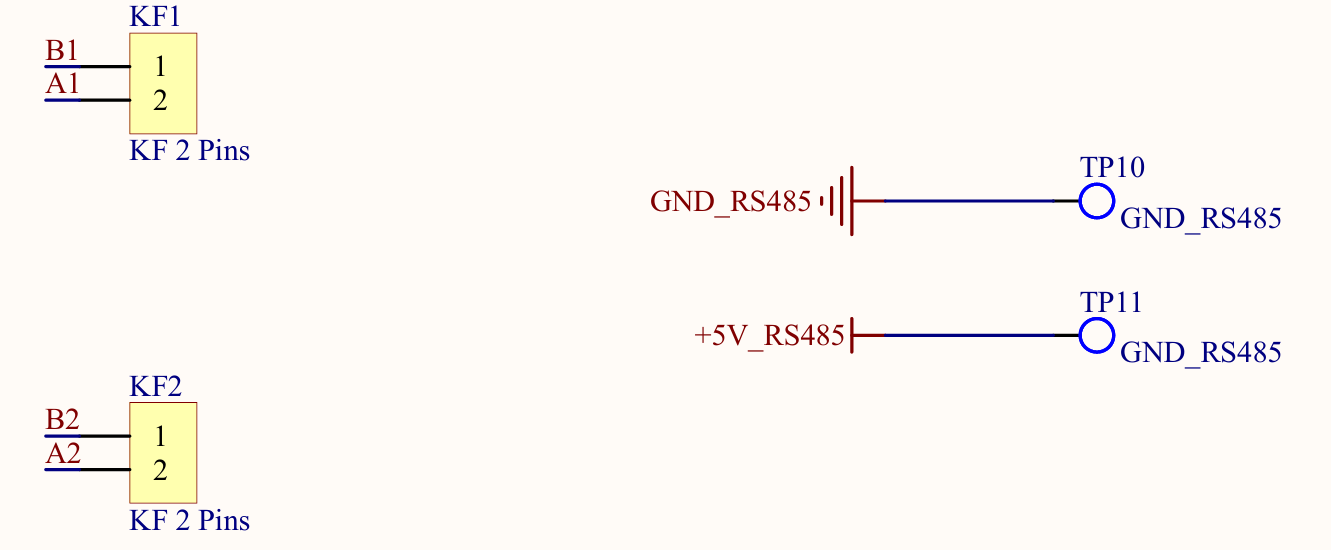
\includegraphics[width=0.6\textwidth]{image/rs485_port.png}
    \caption{khối cổng giao tiếp RS485}
    \label{fig:rs485_port}
\end{figure}
\begin{figure}[H]
    \centering
    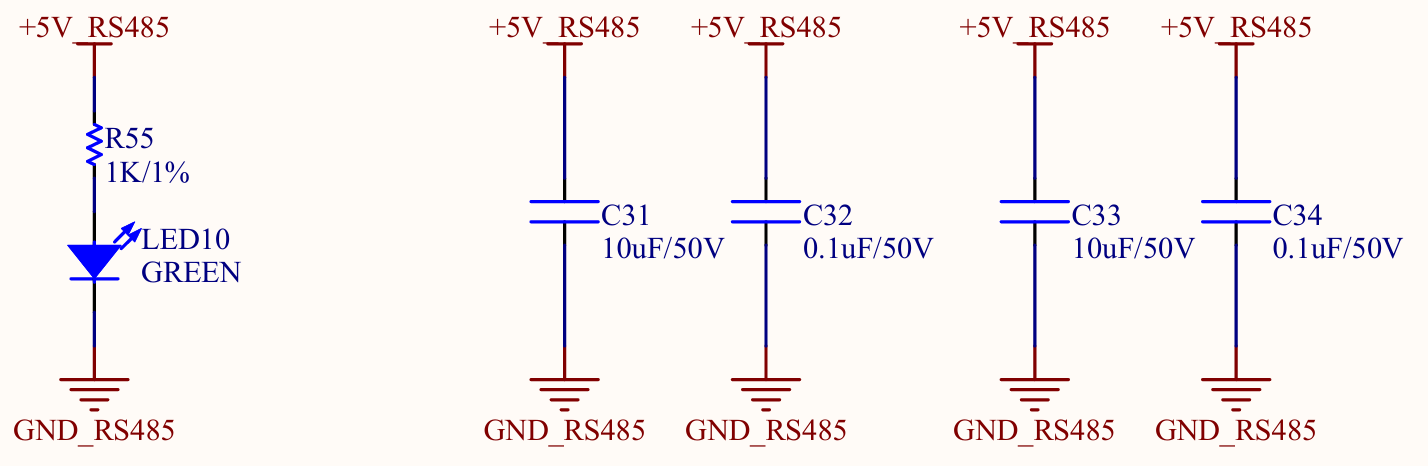
\includegraphics[width=0.6\textwidth]{image/rs485_filter.png}
    \caption{khối lọc nguồn đầu vào và LED báo nguồn}
    \label{fig:rs485_filter}
\end{figure}
Các tụ điện lọc nguồn đầu vào giúp điện áp cấp cho các thành phần trong mạch hoạt động ổn định.
\subsubsection{Thiết kế khối EEPROM và RTC}
\begin{figure}[H]
    \centering
    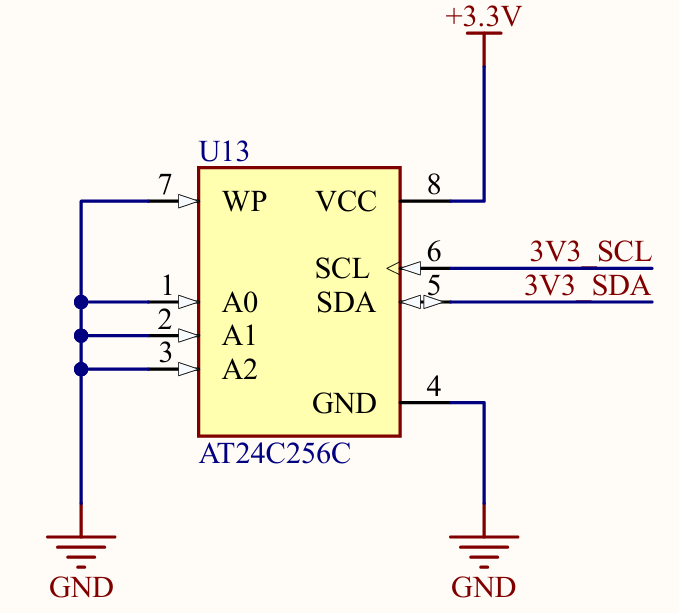
\includegraphics[width=0.5\textwidth]{image/eeprom.png}
    \caption{khối bộ nhớ EEPROM}
    \label{fig:eeprom}
\end{figure}
Mạch có tích hợp sử dụng bộ nhớ EEPROM 256Kbit, giúp lưu trữ các thông tin liên quan tới cấu hình wifi cho vi điều khiển, sử dụng giao tiếp I2C với tốc độ 100KHz,
giúp giảm tải lên bộ nhớ Flash của vi điều khiển.
\begin{figure}[H]
    \centering
    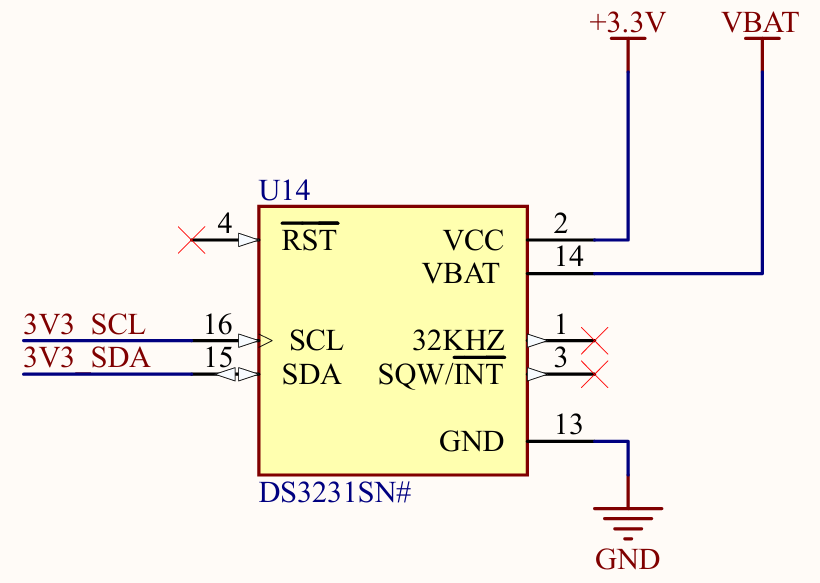
\includegraphics[width=0.5\textwidth]{image/rtc.png}
    \caption{khối RTC}
    \label{fig:rtc}
\end{figure}
Khối RTC giúp lưu trữ thông tin thời gian, khi vi điều khiển kết nối được với Internet thì sẽ lấy thời gian từ NTP sau đó lưu vào trong RTC và sử dụng Pin CR2302 tích hợp,
giúp IC vẫn có thể hoạt động ngay cả khi nguồn chính bị mất, giao tiếp I2C 100KHz sử dụng chung bus với bộ nhớ EEPROM. Khi vi điều khiển không thể kết nối được với internet thì sẽ sử dụng thời gian lưu sẵn trong khối RTC.

\begin{figure}[H]
    \centering
    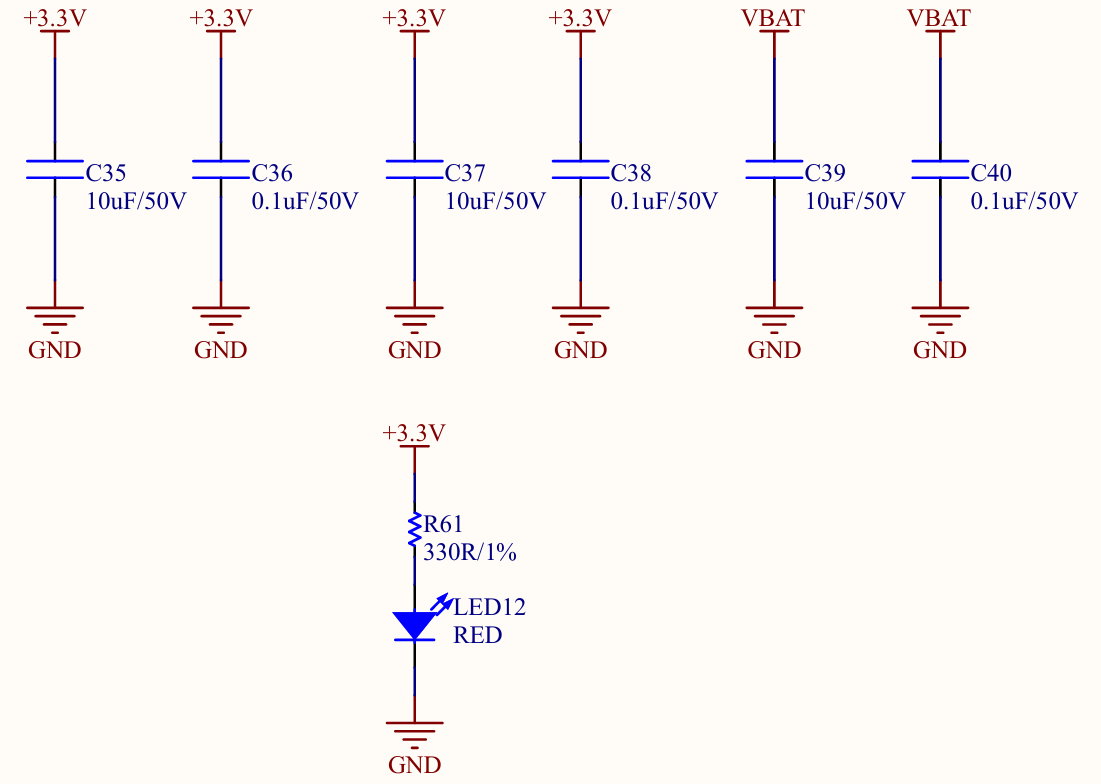
\includegraphics[width=0.6\textwidth]{image/rtc_filter.png}
    \caption{khối lọc nguồn đầu vào cho EEPROM và RTC}
    \label{fig:rtc_filter}
\end{figure}
Thực hiện thiết kế khối lọc nguồn đầu vào dùng chung cho cả nguồn nuôi EEPROM và RTC .
\subsubsection{Thiết kế khối giao tiếp với người dùng}
\begin{figure}[H]
    \centering
    % Hình thứ nhất
    \begin{minipage}{0.45\textwidth}
        \centering
        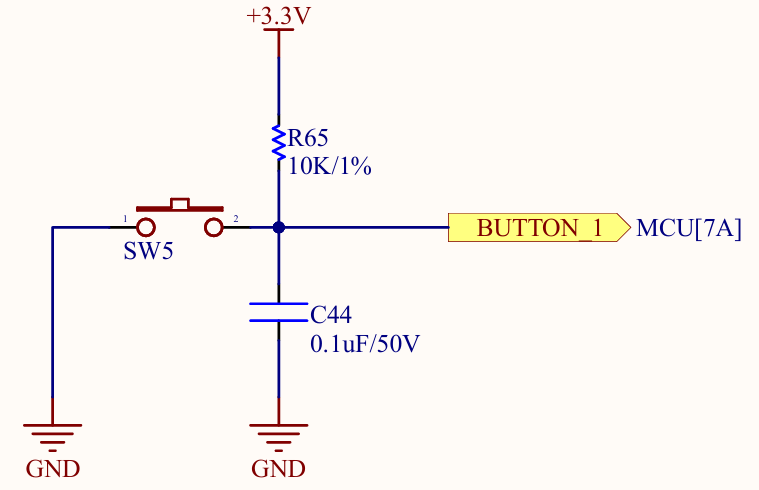
\includegraphics[width=\linewidth]{image/but1.png}
    \end{minipage}
    \hspace{0.05cm} % Khoảng cách giữa các hình
    % Hình thứ hai
    \begin{minipage}{0.45\textwidth}
        \centering
        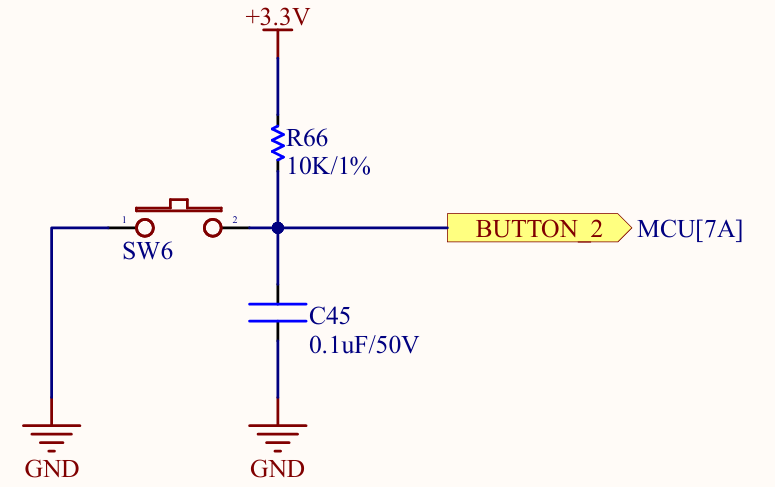
\includegraphics[width=\linewidth]{image/but2.png}
    \end{minipage}
    \hspace{0.05cm} % Khoảng cách giữa các hình
    % Hình thứ ba
    \begin{minipage}{0.45\textwidth}
        \centering
        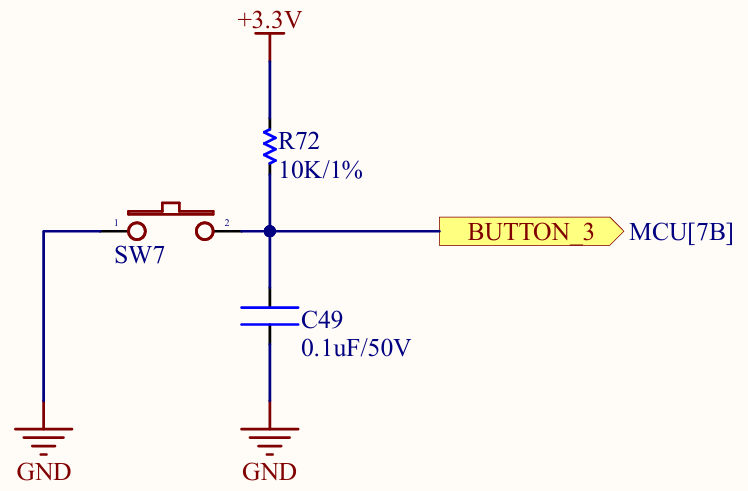
\includegraphics[width=\linewidth]{image/but3.png}
    \end{minipage}

    \caption{khối nút nhấn tương tác với người dùng}
    \label{fig:ba_hinh_modbus}
\end{figure}
\begin{figure}[H]
    \centering
    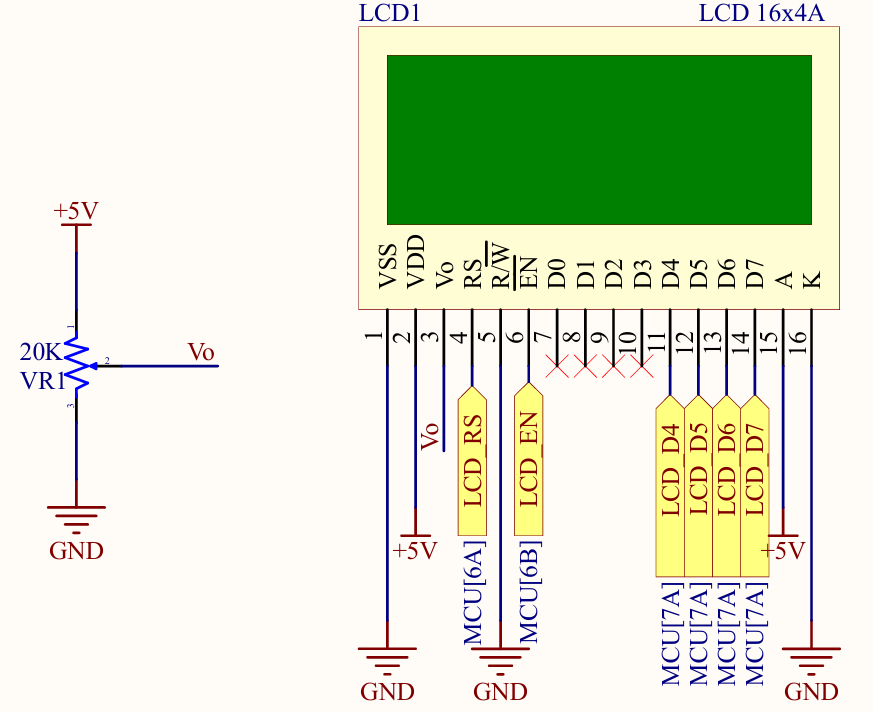
\includegraphics[width=0.6\textwidth]{image/lcd.png}
    \caption{màn hình LCD hiển thị}
    \label{fig:lcd}
\end{figure}
Mạch tích hợp ba nút nhấn lập trình cho phép người dùng có thể tương tác với thiết bị.

Màn hình LCD 16x04 hiển thị các thông tin cấu hình hiện có trên thiết bị, các tính năng của nút nhấn giúp tương tác và hiển thị thông tin trên LCD,
giúp người dùng có thể điều chỉnh thông số và có thể cấu hình thông số tại chỗ mà không cần phải kết nối với máy tính.

Biến trở 20K Ohm giúp điều chỉnh hiển thị độ tương phản trên màn hình LCD.